\section{Starting}
\label{sec:startup_starting}

After the previous steps have been completed and the database is finalized, the 'Start' button can be pressed to continue. \\

\begin{figure}[H]
  \center
    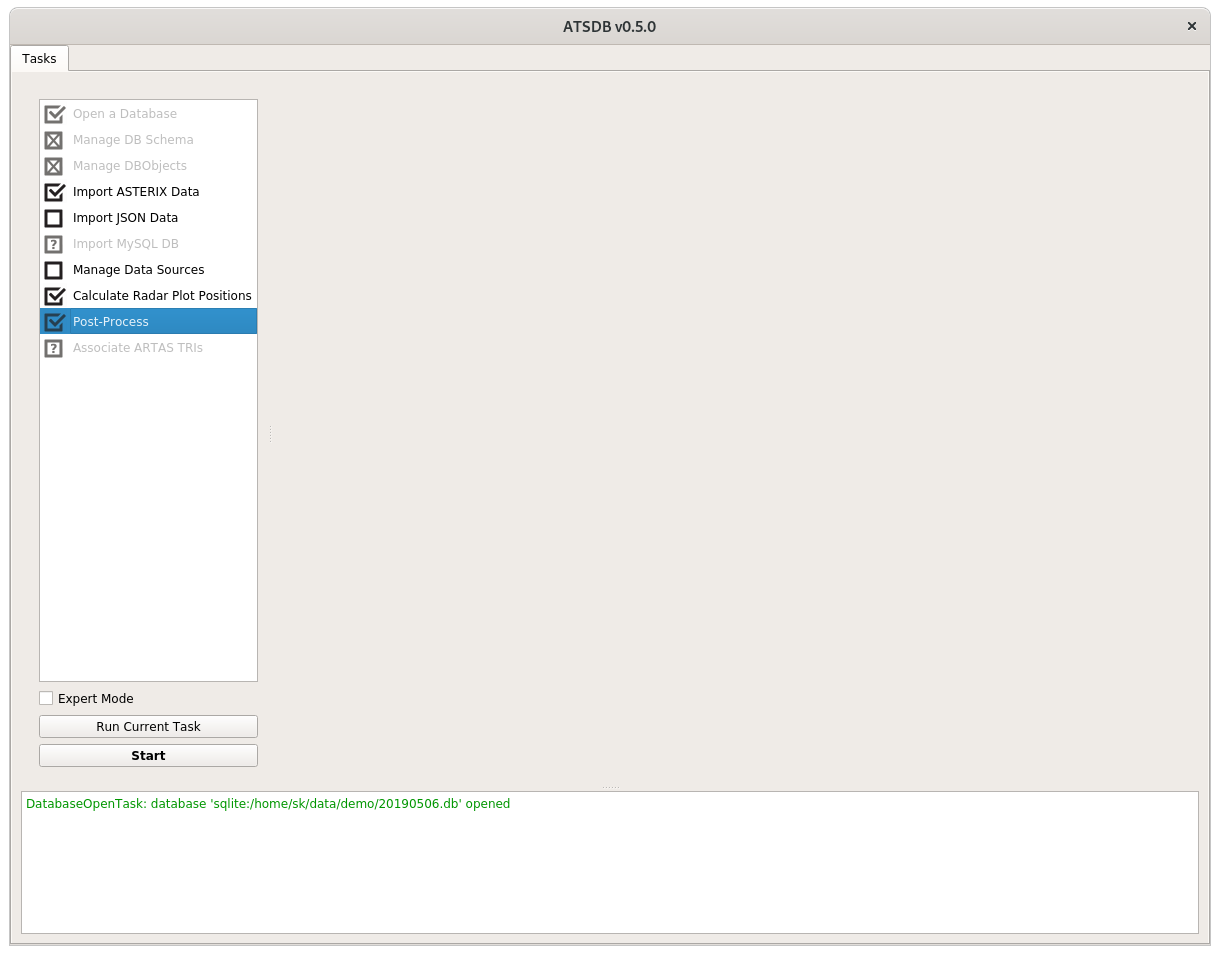
\includegraphics[width=9cm,frame]{../screenshots/start.png}
  \caption{Starting}
\end{figure}

When a database is opened the first time, a post-processing will be performed automatically. 

\subsection{Postprocessing}
When a database is imported, some information that eases usage of the software does not exist. This information is generated once during a post-processing step, which is automatically performed the first opening of a new database. If wanted, it can always performed using the 'Force post-processing' checkbox.

\begin{figure}[H]
  \hspace*{-2cm}
    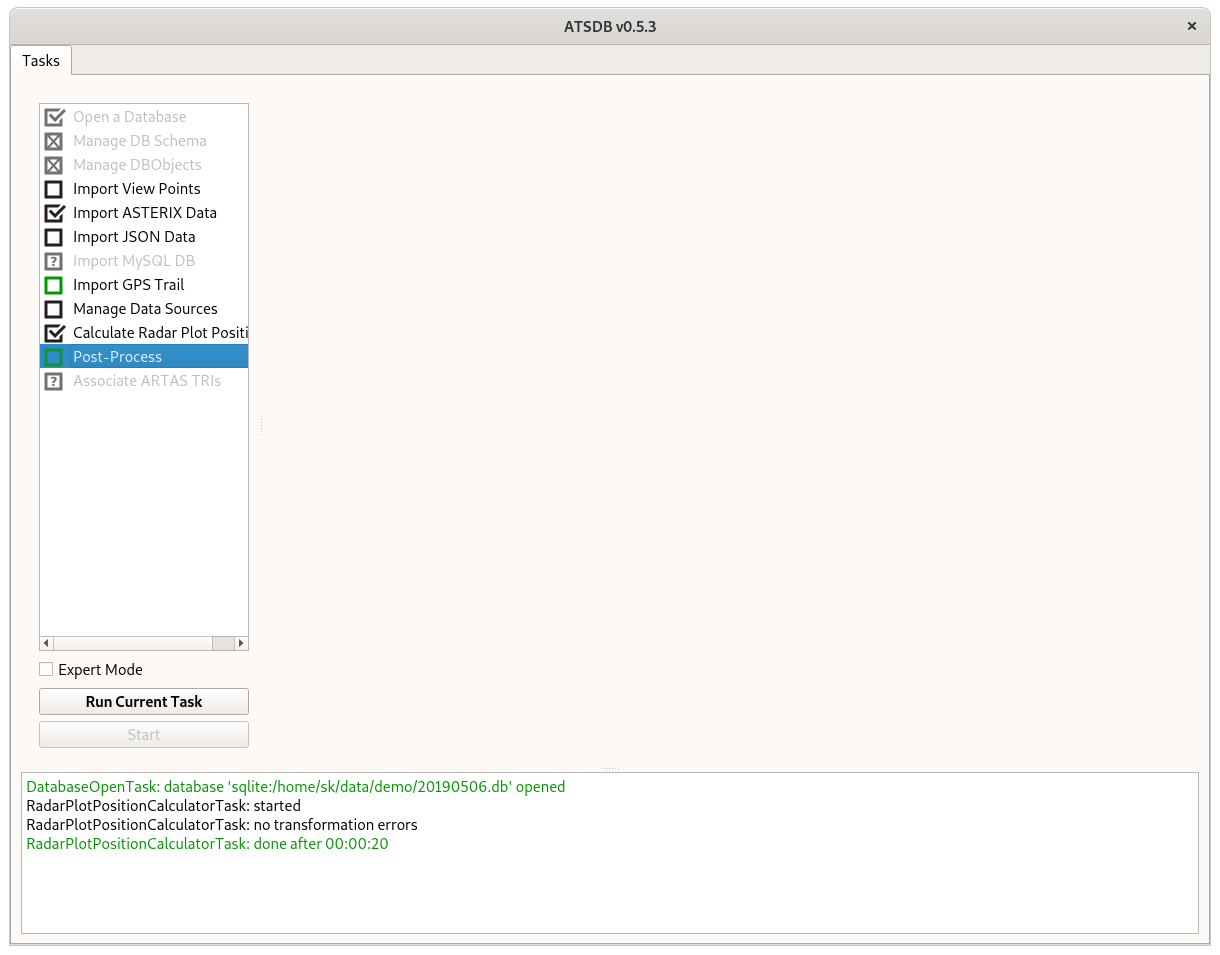
\includegraphics[width=18cm,frame]{../screenshots/db_postprocessing.png}
  \caption{Post-processing a database}
  \label{fig:db_postprocessing}
\end{figure}

The following information is generated and stored in the database:

\begin{itemize}  
\item List of all active data sources for all DBOs
\item List with all minima/maxima for all variables of all DBOs
\end{itemize}

This step has to be performed only once for each database, and may take up to a few minutes for large datasets. \\


\includegraphics[width=0.5cm]{../../data/icons/hint.png} Please \textbf{note} that during this step, no DBO data itself is changed, but only additional information is generated and stored in separate database tables.
